\subsection{Estudo de anteparo de proteção para a chama}
Quando não é possível, em uma passada única, atraves\-sar completamente a
superfície ao realizar o \textit{coating}, coloca-se uma placa de sacrifício, pois, como
menciona\-do em \ref{sec::desc_hvof}, não é permitido para ou trocar de direção
subre a superfície.

Para evitar a necessidade de sobrepôr placas de sacrifício sobre as pás da
turbina, que podem estar em posição de difícil acesso, foi criado o conceito de
\textit{shutter}. Este consiste em um antepero a ser posicionado entre a chama e
a superfície, porém, diferente da placa de sacrifício, deve ficar preso à
pistola de metalização e ser atuado.

A pistola de metalização propaga uma chama de $3000^o$ (\ref{sec::desc_hvof}), assim,
a parte da pistola com maior aquecimento, que é o canhão, é fabricado em
cobre-cromo e é refrigerada por um sistema de circulação de água
gelada. A chapa de sacrifício, por outro lado, fica pouco tempo em contato com
a chama e é constituída de um aço qualquer sem sistema de refrigeração
\ref{sec::desc_hvof}.

Quando se planeja submeter o anteparo à temperatu\-ra extrema de $3000^o$ da
chama, sem um sistema de refrigeração, torna-se necessário o uso de materia\-is
especiais para suportar essa temperatura. Para isso existem materiais
aeroespaciais, conhecidos como Ultra-high-temperature ceramics (UHTCs) ou
cerâmi\-cas de temperaturas ultra-altas, em tradução livre. Esse grupo de
materiais possui diversas sub-famílias com densidades e resistência mecânicas
diferentes. Para os cálculos realizados nessa seção foram consideradas a maior
densidade e menor resistência mecânica entre os compostos das sub-famílias. Ou
seja, foi utilizado aproximadamente \textbf{$15 g/mL$} para a densidade, referente ao
carbeto de tântalo \citep{bansal2005ceramic}. E as características mecânicas
foram referentes ao diboreto de zircônio \citep{diborides}.

Foram desenvolvidos dois conceitos similares para resolver o problema, o \textit{Shutter
Borboleta} e o \textit{Shutter Padrão}, descritos a seguir.

\subsubsection{\textit{Shutter} Borboleta}
\label{borboleta}

Esse primeiro conceito é constituido de um disco disposto antre a chama e a
superfície. O disco possui duas aberturas opostas de $90^o$, por onde a chama da
pistola travessa, e as outras duas regiões de $90^o$ compostas pelo material que
servirá de anteparo para a chama, a fim de evitar o coating da superfície, que
dão o nome ``borboleta'' ao design.
O disco é suportado por um eixo que é rotacionado por um motor afixionado sobre o
corpo da pistola de metalização (figuras \ref{fig::borboleta_aberta} e
\ref{fig::borboleta_fechada}).

\begin{figure}[h!]
\centering
	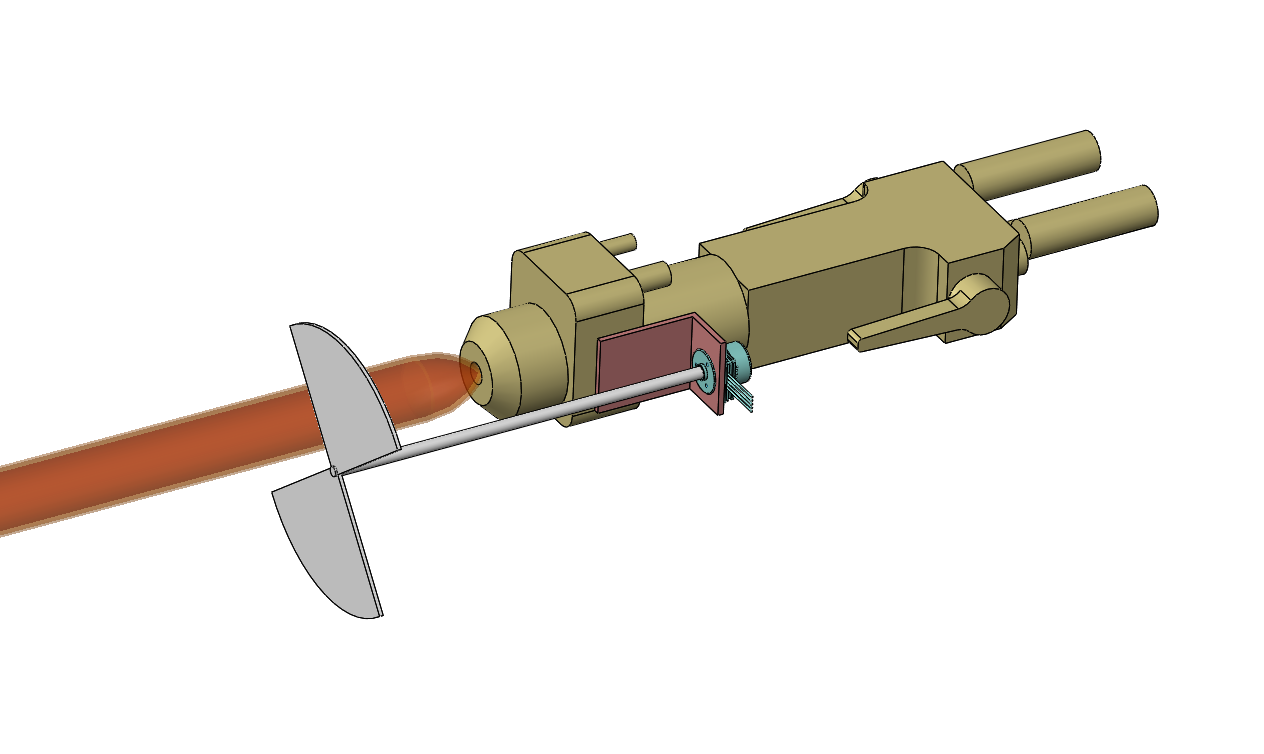
\includegraphics[width=\columnwidth]{figs/estudo/shutter/Shutter_Borboleta_Aberto}
	\caption{\textit{Shutter} Borboleta em posição aberta, permitindo a passagem da chama
	de coating.}
	\label{fig::borboleta_aberta}
\end{figure}

Quando uma das regiões de abertura do \textit{shutter} se encontra na direção da
chama (figura \ref{fig::borboleta_aberta}), esta o atravessa e atinge a
superfície a ser tratada sem sofrer desvios. Para realizar uma mudança de
direção do \textit{coating} ou parada por qualquer motivo, o motor gira o conjunto
eixo/disco e posiciona a região de proteção na direção da chama, o que impede a passagem da
chama (figura \ref{fig::borboleta_fechada}).

\begin{figure}[h!]
\centering
	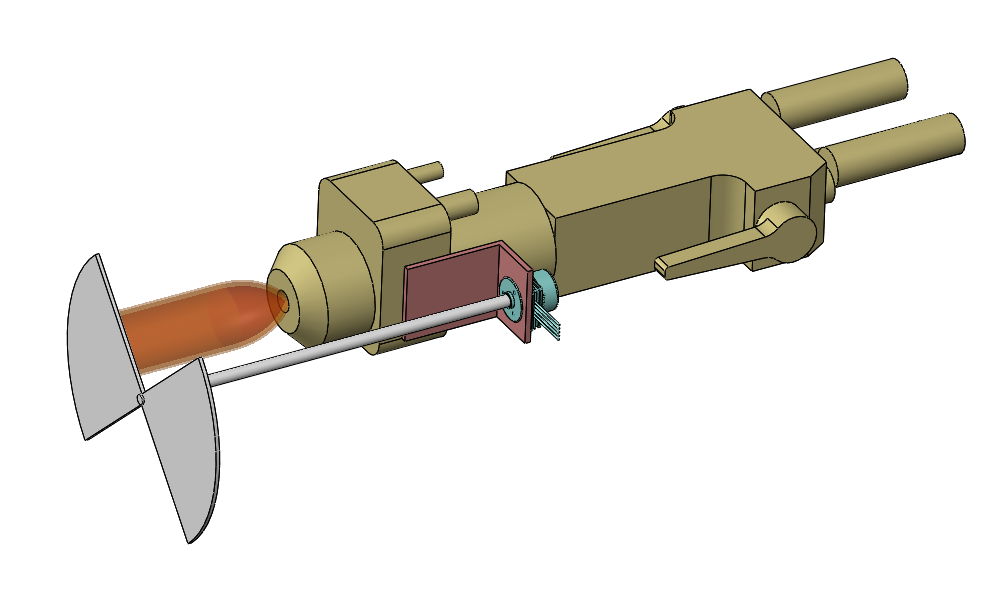
\includegraphics[width=\columnwidth]{figs/estudo/shutter/Shutter_Borboleta_Fechado}
	\caption{\textit{Shutter} Borboleta em posição fechada, evitando a passagem da chama
	de coating, agindo como anteparo de forma similar à chapa de sacrifício.}
	\label{fig::borboleta_fechada}
\end{figure}

Para dimensionamento do eixo e da borboleta foram considerados os seguintes
parâmetros:

\[\rho = 15 g/mL\]
\[v_{close} = 40 m/min\]
\[d_{flame} = 33mm\]
\[L = 20mm\]

Onde $\rho$ é a densidade do do material do \textit{shutter}, $v_{close}$ a
velocidade de fechamento sobre a chama, $d_{flame}$ o diâmetro da chama e $L$ o
comprimento do eixo. Além desses parâmetros, foram utilizadas informações
mecânicas como módulos de elasticidade e limites de escoamentos típicos de aço.

Para a escolha do comprimento do eixo, o objetivo foi posicionar o
\textit{shutter} a meio caminho da pistola à superfície, e mantendo $10cm$ de
distância entre a posição do motor e a saída da chama (a fim de evitar
exposição ao calor intenso). Durante o dimensionamento do shutter foi
considerado um valor de segurança para o diâmetro da chama como o dobro do
diâmetro real.

A partir desses dados chegamos aos seguintes requisitos para o sistema:

\[ r = 80 mm\]
\[ \epsilon = 5 mm\]
\[ \omega = 160 rpm\]
\[ {Pot}_{min} = 5 W \]
\[ \tau_{min} = 420 mNm \]
\[ Pot_{\tau} = 7 W \]
\[ d_{eixo} = 7 mm\]

Onde $r$ é o raio do \textit{shutter}, $\epsilon$ sua espessura, o que acarreta
um peso de $750g$ para o \textit{shutter}.

Há, também, $\omega$ que é a velocidade de rotação que o motor precisa alcançar,
$Pot_{min}$ sua potência mínima e $\tau_{min}$ seu torque mínimo necessário.
$Pot_{\tau}$ é a potência mínima necessária caso o torque mínimo ($\tau_{min}$)
for para ser mantido durante todo o percurso de fechar/abrir a passagem da
chama. E, por fim, $\d_{eixo}$ é o diâmetro necessário do eixo para suportar a
pressão da chama.

Foram pesquisados motores industriais de pequenas dimensões (menos de 300g),
porém não foram encontrados motores capazes de suprir o torque necessário. Como
são facilmente encontrados motores que satisfazem as restrições de potência,
existem redutores de dimensões diminutas que podem ser acoplados ao motor para
fazê-lo trabalhar na faixa de torque necessária.


\subsubsection{Shutter Padrão}

O \textit{Shutter} Padrão é composto por uma pequena chapa quadrada que é
posicionada entre a pistola e a superfície pela atuação de um motor. O motor é
conectado à chapa por quatro astes presas em suas extermidades, como mostram as
figuras \ref{fig::padrao_aberto} e \ref{fig::padrao_fechado}.

\begin{figure}[h!]
\centering
	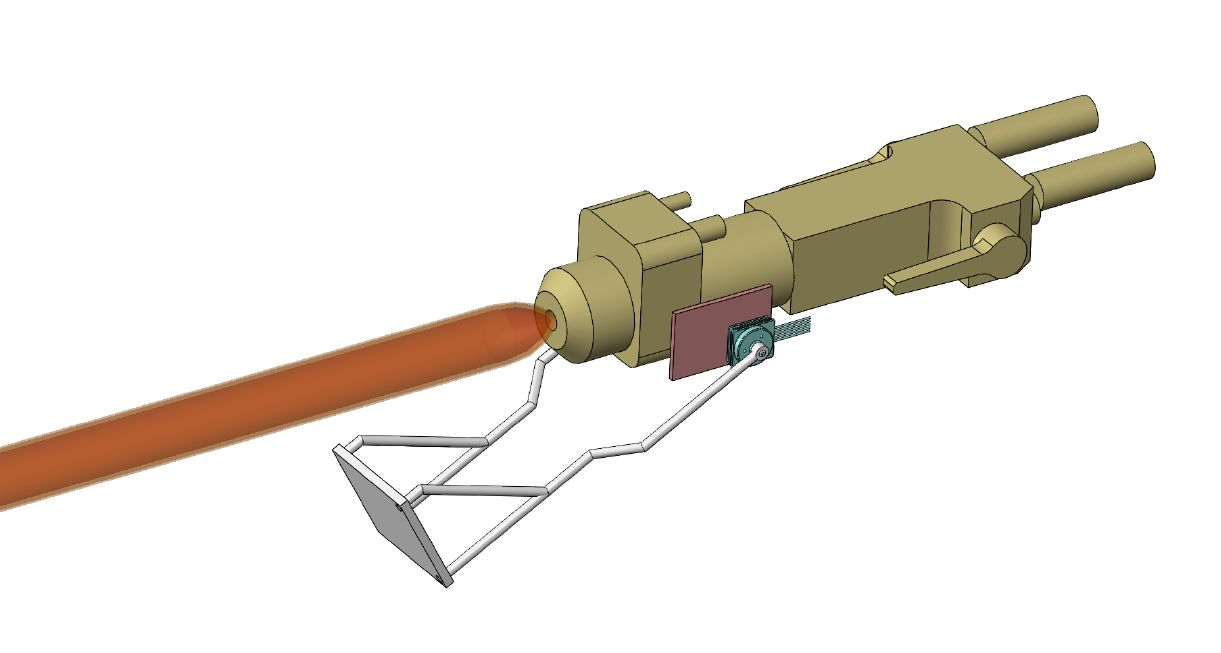
\includegraphics[width=\columnwidth]{figs/estudo/shutter/Padrao_aberto}
	\caption{\textit{Shutter} Padrão em posição aberta, permitindo a passagem da chama
	de coating.}
	\label{fig::padrao_aberto}
\end{figure}

Quando a chapa se encontra fora do eixo da chama dizemos que
o \textit{shutter} está aberto (figura \ref{fig::padrao_aberto}), permitindo que o \textit{coating}
seja realizado normalmente. Na necessidade de impedir a passagem da chama, o
motor atua sobre as astes guiando a chapa para servir de anteparo à chama, é a
posição fechada (figura \ref{fig::padrao_fechado}).

\begin{figure}[h!]
\centering
	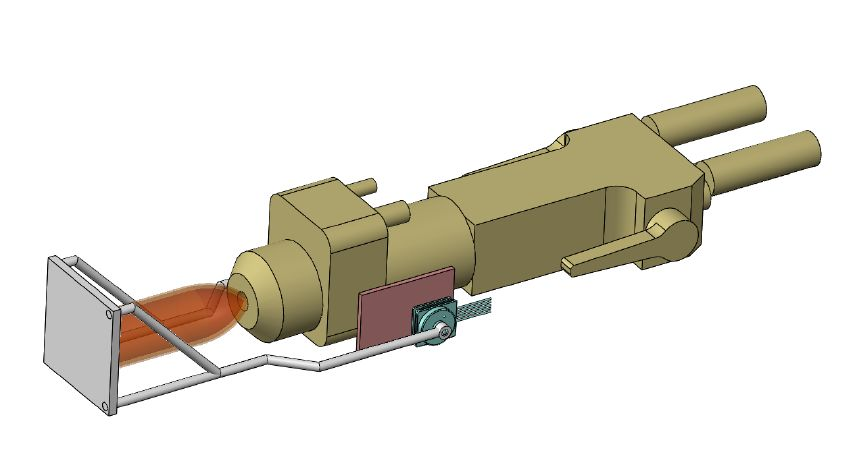
\includegraphics[width=\columnwidth]{figs/estudo/shutter/Padrao_fechado}
	\caption{\textit{Shutter} Padrão em posição fechada, evitando a passagem da
	chama de coating, agindo como anteparo de forma similar à chapa de sacrifício.}
	\label{fig::padrao_fechado}
\end{figure}

Para calcular os requistos do motor e da chapa foram considerados os mesmos
valores utilizados no \textit{shutter} borboleta (\ref{borboleta}). Sendo a
escolha do comprimento do eixo e o diâmetro de segurança da chama feitos
seguindo os mesmo preceitos também lá descritos.

A partir desses dados chegamos aos seguintes requisitos para o sistema:

\[ l = 66 mm\]
\[ \epsilon = 5 mm\]
\[ \omega = 32 rpm\]
\[ {Pot}_{min} = 2 W \]
\[ \tau_{min} = 920 mNm \]
\[ Pot_{\tau} = 3 W \]


Onde $l$ é o lado da chapa do \textit{shutter}, $\epsilon$ sua espessura, o que
acarreta um peso de $350g$ para o \textit{shutter}.

A velocidade de rotação que o motor precisa alcançar foi nomeada $\omega$, sua
potência mínima $Pot_{min}$  e seu torque mínimo necessário $\tau_{min}$.
$Pot_{\tau}$ é a potência mínima necessária para que o torque mínimo
($\tau_{min}$) consiga ser mantido durante todo o percurso de fechar/abrir.

Assim como para o \textit{shutter} borboleta não foram encontrados motores
capazes de suprir o torque necessário. E a solução pelo uso de redutores de
dimensões diminutas pode ser facilmente aplicada devido à baixa potência
requerida.
